%
% File acl2018.tex
%
%% Based on the style files for ACL-2017, with some changes, which were, in turn,
%% Based on the style files for ACL-2015, with some improvements
%%  taken from the NAACL-2016 style
%% Based on the style files for ACL-2014, which were, in turn,
%% based on ACL-2013, ACL-2012, ACL-2011, ACL-2010, ACL-IJCNLP-2009,
%% EACL-2009, IJCNLP-2008...
%% Based on the style files for EACL 2006 by 
%%e.agirre@ehu.es or Sergi.Balari@uab.es
%% and that of ACL 08 by Joakim Nivre and Noah Smith

\documentclass[11pt,a4paper]{article}
\usepackage[hyperref]{acl2019}
\usepackage{times}
\usepackage{latexsym}
\usepackage{url}
\usepackage{graphicx}
\usepackage{booktabs}

\aclfinalcopy % Uncomment this line for the final submission
%\def\aclpaperid{***} %  Enter the acl Paper ID here

%\setlength\titlebox{5cm}
% You can expand the titlebox if you need extra space
% to show all the authors. Please do not make the titlebox
% smaller than 5cm (the original size); we will check this
% in the camera-ready version and ask you to change it back.

\newcommand\BibTeX{B{\sc ib}\TeX}

\newcommand{\dpcomment}[1]{\textcolor{green}{[#1 --deric]}}
\newcommand{\jbcomment}[1]{\textcolor{orange}{[#1 --josh]}}

\title{Syntactically Informed Natural Language Inference}

\author{
  Deric Pang \quad
  Joshua Bean \\
  Paul G. Allen School of Computer Science \& Engineering \\
  University of Washington \\
  Seattle, WA, USA \\
  {\tt \{dericp, jbean96\}@cs.washington.edu} \\
}

\date{}

\begin{document}
\maketitle
\begin{abstract}
This project explores methods for improving performance on the task of natural language inference by incorporating syntactic information. Specifically we modify the decomposable attention neural network \citep{Parikh2016-em} by incorporating encoded syntax parses of the input statements at different layers of the network. We supplement these experiments by using different syntax parsers including pre-trained constituency and dependency parsers as well as a constituency parser trained separately for this task. 
\end{abstract}

\section{Introduction}

Natural language inference (NLI) is the task of characterizing entailment and
contradiction relationships between texts. We improve NLI models by adding syntactic
features into existing models.
We will primarily investigate the well-known decomposable attention (DA) neural
network \citep{Parikh2016-em}

In general, most NLI tasks are formulated as characterizing the relationship
between a pair of sequences---a premise and a hypothesis. An NLI model should
predict whether the hyothesis is entailed by the premise, contradicts the
premise, or is neutral to the premise.

We extend the decomposable attention (DA) model by \citet{Parikh2016-em}
incorporating syntactic features.
\dpcomment{Include brief summary of contributions here.}
The DA model obtained state-of-the-art results on the
SNLI \citep{Bowman2015-is} dataset at its time of publication while using
drastically fewer parameters than previous NLI models.
We primarily
evaluate on the domain specific Scitail \citep{Khot2018-th} for both its
smaller size and lack of annotation artifacts when compared to SNLI
\citep{Gururangan2018-lj}.

\section{Syntactic Entailment}

In previous work, we created the syntail-v1 model whose architecture is shown
in figure~\ref{figure:v1}.  We have obtained mixed results as shown in
table~\ref{table:v1-accuracies} when naively incorporating syntactic
information into the DA model.

Without ELMo, syntail-v1 improves an impressive 8.4\% in test accuracy over the
baseline decomposable attention model on the SciTail dataset. However, once
ELMo is added to the model, almost the exact opposite occurs. Adding syntactic
information decreases test accuracy by 6.7\% with ELMo.

\begin{table}[h]
  \resizebox{0.45\textwidth}{!}{
  \begin{tabular}{c c c c}
    \toprule
    Model & Embedding & Train Acc. & Test Acc. \\
    \midrule
    DA & GLoVe 6b 300d & 89.4\% & 70.1\% \\
    \textbf{Syntail-v1} & \textbf{GLoVe 6b 300d} & \textbf{92.1\%}
                        & \textbf{78.5\%} \\
    DA & ELMo & 98.4\% & 78.0\% \\
    \textbf{Syntail-v1} & \textbf{ELMo} & \textbf{88.8\%} & \textbf{71.3\%} \\
    \bottomrule
  \end{tabular}}
  \caption{Syntail-v1 and DA model accuracies on the SciTail dataset.}
\label{table:v1-accuracies}
\end{table}

\section{Models}

The syntactic entailment model is derived from the decomposable attention model for natural language inference described by \citet{Parikh2016-em}. In the initial iteration of the network, syntax is not incorporated until the very last feed-forward layer. This means that syntax is not considered when calculating attention between the premise and the hypothesis. We speculated that by introducing syntax to the network prior to calculating attention we would see better results as the syntax would help influence the attention calculations and reveal the most important phrases of each input statement.

In the ``V3" model, we perform the same initial step of embedding the premise and hypothesis and expanding their dimensions (through a fully-connected layer) prior to attention. However, instead of calculating our similarity matrix using solely the embedded hypothesis and premise vectors as input, we also provide the encoded syntax parses of both inputs. The concatenation of these four vectors is used to derive the similarity matrix which is then utilized in the attention computations between the premise and hypothesis.

With the ``V5" model we tried to incorporate the computed syntax of the inputs even earlier. Instead of concatenating the encoded syntax parses with the embedded inputs and using that as input for the computation of the similarity matrix, we concatenated the syntax parses with their respective inputs and passed that through the first fully-connected layer. The two resulting vectors representing the embedded inputs with syntactic information are then used to compute the similarity matrix.

Our ``V7" model took an additional step of learning weights for the encoded syntax parses by passing the vectors through an additional fully-connected layer before introducing them into the rest of the network. This model was built on top of the ``V3" model such that the weighted syntax parses are concatenated with the embedded premise and hypothesis statements when deriving the similarity matrix.

Supplemental variations were done on top of these restructures of the network. One of the variations that we introduced was a retrained constituency parser. By retraining the constituency parser on the Penn Treebank dataset \citep{marcus1993building} we could change the dimensions of the encoded syntax vectors to better fit with our models. Additionally, we experimented with training our models using the dependency parser model derived by \citet{dozat2016deep} to see if the different types of encoded parses influenced the performance of the network.

\section{Proposed Methods}
\label{methods}

We plan to use state-of-the-art constituency \citep{Stern2017-co} and
dependency \citep{Dozat2016-gs} parsers to investigate if incorporating
syntactic features improves the performance of the DA model. Additionally, we
hope to understand how syntactic features interact with contextual word
embeddings like ELMo \citep{Peters2018-fz} and BERT \citep{Devlin2018-qc} in a
task like NLI. It is unclear from previous work whether contextual word
embeddings benefit from additional syntactic information or if something like
ELMo can already adequately capture this information.

We will first investigate different ways of incorporating syntactic
information. \citet{Pang2018-syntail} use a constituency parser to obtain an
encoding of the premise and hypothesis that is in the final fully-connected
layer of the DA model. We believe that incorporating syntactic features earlier
in the pipeline, especially before the premise and hypothesis are attended over
one another, should improve performance.

We will then investigate different model architectures under a multi-task
training objective where the jointly learns to both parse and predict
entailment relationships.

\begin{figure}[h]
  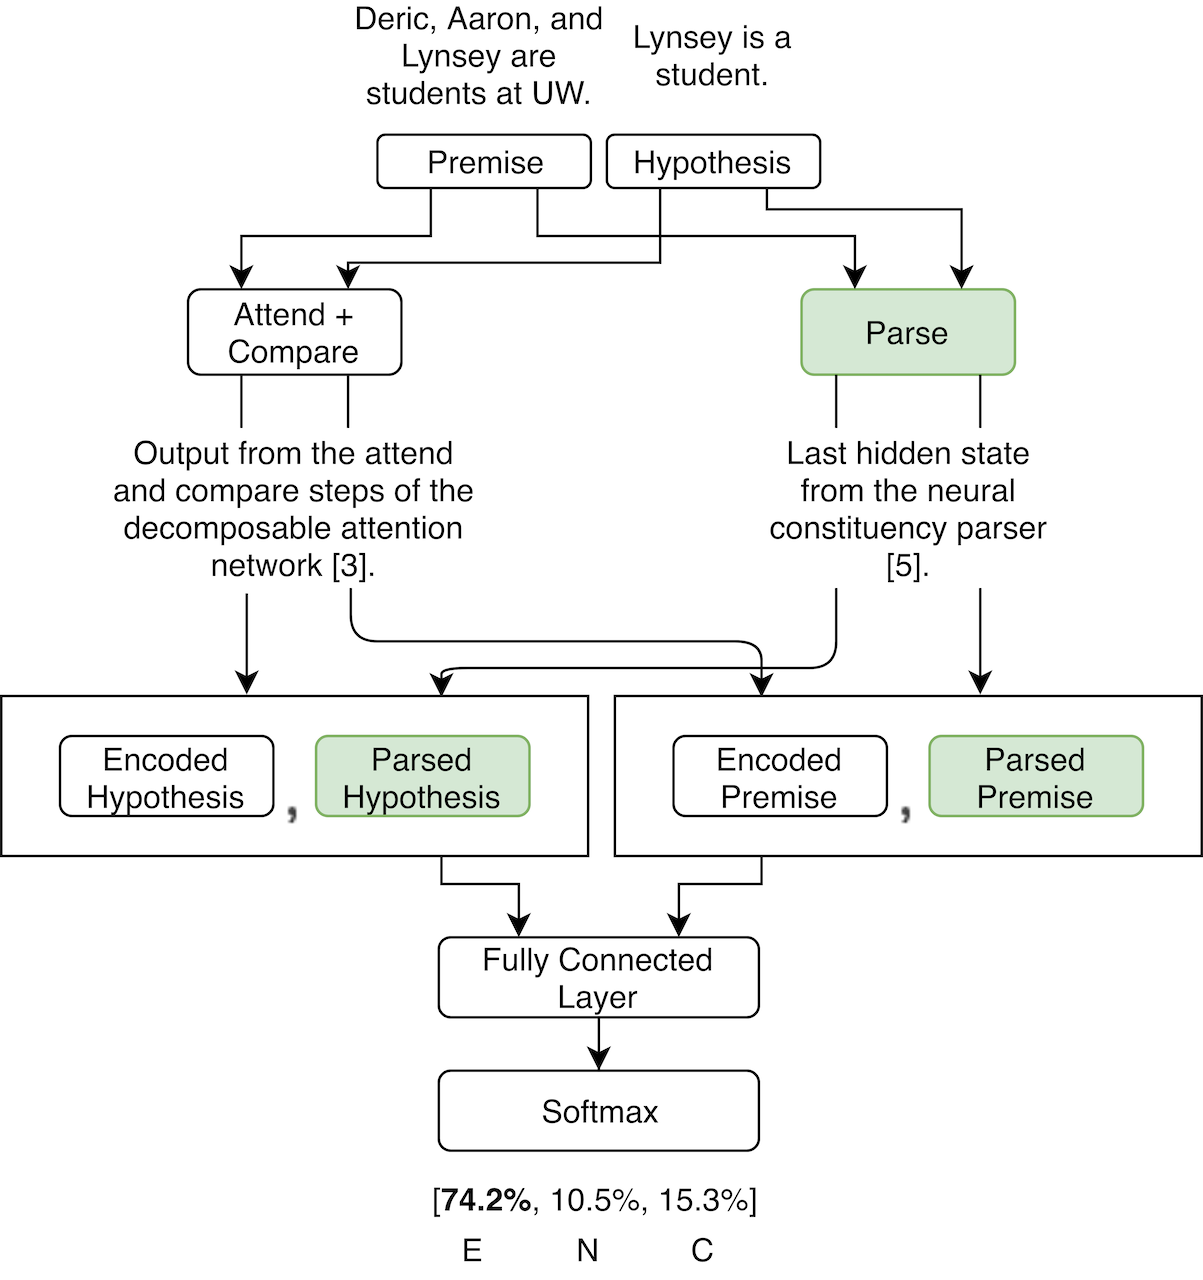
\includegraphics[width=0.45\textwidth]{v1}
  \caption{A simple method of incorporating syntax into the decomposable
    attention model.}
\label{figure:v1}
\end{figure}

\section{Expected Outcomes}

We will compare our models to the DA model as well as syntail-v1. We hope to
evaluate our models on many diverse datasets as stated in section
~\ref{methods}.

We expect that one of our modeling ideas will produce results that improve on
the DA and syntail-v1 models. In the best case, we will show that syntax is
crucial to building an accurate NLI system.

\section{Challenges}

The first challenge involved in our project will be to modify syntail-v1
so that syntactic information is incorporated much earlier. It will also take
significant time to investigate the best parsers to use for our model.
After, we will write a new model under a multi-task training setup, which we
anticipate will be a significant implementation challenge.

We expect to require significant compute power and time to adequately fine-tune
and evaluate our models. Contextual word embeddings are especially costly to
train, and the mixing ratio in a multi-task setup is well-known to be
difficult to tune.

\bibliographystyle{acl_natbib}
\bibliography{main}

\end{document}
